\printconcepts

\exercise{T/F: An ``optimization problem'' is essentially an ``extreme values'' problem in a ``story problem'' setting.}{T}

\exercise{T/F: This section teaches one to find the extreme values of function that have more than one variable.}{F}

\printproblems

\exercise{Find the maximum product of two numbers (not necessarily integers) that have a sum of 100.}{2500; the two numbers are each 50. }

\exercise{Find the minimum sum of two positive numbers whose product is 500.}{The minimum sum is $2\sqrt{500}$; the two numbers are each $\sqrt{500}$.}

\exercise{Find the maximum sum of two positive numbers whose product is 500.}{There is no maximum sum; the fundamental equation has only 1 critical value that corresponds to a minimum.}

\exercise{Find the maximum sum of two numbers, each of which is in $[0,300]$ whose product is 500.}{The only critical point of the fundamental equation corresponds to a minimum; to find maximum, we check the endpoints. 

If one number is 300, the other number $y$ satisfies $300y = 500$; $y = 5/3$. Thus the sum is $300+5/3$. 

The other endpoint, 0, is not feasible as we cannot solve $0\cdot y = 500$ for $y$. In fact, if $0<x<5/3$, then $x\cdot y = 500$ forces $y>300$, which is not a feasible solution. 

Hence the maximum sum is $301.\overline{6}$.}

\exercise{Find the maximal area of a right triangle with hypotenuse of length 1.}{Area = 1/4, with sides of length $1/\sqrt{2}$.}

\exercise{A rancher has 1000 feet of fencing in which to construct adjacent, equally sized rectangular pens. What dimensions should these pens have to maximize the enclosed area?

\noindent\begin{minipage}{\linewidth}
\centering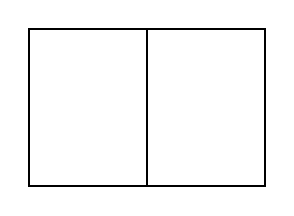
\begin{tikzpicture}
\draw [draw={\colorone},thick](0,0) rectangle (3,2);
\draw [draw={\colorone},thick](1.5,0) -- (1.5,2);
\end{tikzpicture}
\end{minipage}
}{Each pen should be $500/3\approx 166.67$ feet by 125 feet.}

\exercise{A standard soda can is roughly cylindrical and holds 355cm$^3$ of liquid. What dimensions should the cylinder be to minimize the material needed to produce the can? Based on your dimensions, determine whether or not the standard can is produced to minimize the material costs.}{The radius should be about $3.84$cm and the height should be $2r=7.67$cm. No, this is not the size of the standard can.}

\exercise{Find the dimensions of a cylindrical can with a volume of 206in$^3$ that minimizes the surface area.

The ``\#10 can''is a standard sized can used by the restaurant industry that holds about 206in$^3$ with a diameter of 6 2/16in and height of 7in. Does it seem these dimensions where chosen with minimization in mind?
}{The radius should be about $3.2$in and the height should be $2r=6.4$in. As the \#10 is not a perfect cylinder (with extra material to aid in stacking, etc.), the dimensions are close enough to assume that minimizing surface area was a consideration.}

\exercise{The United States Postal Service charges more for boxes whose combined length and girth exceeds 108'' (the ``length'' of a package is the length of its longest side; the girth is the perimeter of the cross section, i.e., $2w+2h$). 

What is the maximum volume of a package with a square cross section ($w=h$) that does not exceed the 108'' standard? 
}{The height and width should be $18$ and the length should be $36$, giving a volume of $11,664$in$^3$.}

\exercise{The strength $S$ of a wooden beam is directly proportional to its cross sectional  width $w$ and the square of its height $h$; that is, $S = kwh^2$ for some constant $k$. 

\noindent\begin{minipage}{\linewidth}
\centering
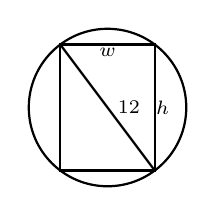
\begin{tikzpicture}
\draw [draw={\colorone},thick](0,0) circle (1cm);
\draw [draw={\colorone},thick](-.6,.8) -- node [pos=.5,right,color=black] {\scriptsize $12$} (.6,-.8);
\draw [draw={\colorone},thick](-.6,-.8) rectangle (.6,.8);
\draw (.7,0) node {\scriptsize $h$} (0,.7) node {\scriptsize $w$};
\end{tikzpicture}
\end{minipage}

Given a circular log with diameter of 12 inches, what sized beam can be cut from the log with maximum strength?}{$w=4\sqrt{3}$, $h=4\sqrt{6}$}

\exercise{A power line is to be run to an offshore facility in the manner described in \autoref{ex_opt3}. The offshore facility is 2 miles at sea and 5 miles along the shoreline from the power plant. It costs \$50,000 per mile to lay a power line underground and \$80,000 to run the line underwater. 

How much of the power line should be run underground to minimize the overall costs?
}{$5-10/\sqrt{39} \approx 3.4$ miles should be run underground, giving a minimum cost of \$374,899.96.}

\exercise{A power line is to be run to an offshore facility in the manner described in \autoref{ex_opt3}. The offshore facility is 5 miles at sea and 2 miles along the shoreline from the power plant. It costs \$50,000 per mile to lay a power line underground and \$80,000 to run the line underwater. 

How much of the power line should be run underground to minimize the overall costs?
}{The power line should be run directly to the off shore facility, skipping any underground, giving a cost of about \$430,813.}

\exercise{A woman throws a stick into a lake for her dog to fetch; the stick is 20 feet down the shore line and 15 feet into the water from there. The dog may jump directly into the water and swim, or run along the shore line to get closer to the stick before swimming. The dog runs about 22ft/s and swims about 1.5ft/s. 

How far along the shore should the dog run to minimize the time it takes to get to the stick? (Hint: the figure from \autoref{ex_opt3} can be useful.)
}{The dog should run about 19 feet along the shore before starting to swim.}

\exercise{A woman throws a stick into a lake for her dog to fetch; the stick is 15 feet down the shore line and 30 feet into the water from there. The dog may jump directly into the water and swim, or run along the shore line to get closer to the stick before swimming. The dog runs about 22ft/s and swims about 1.5ft/s. 

How far along the shore should the dog run to minimize the time it takes to get to the stick? \textit{\footnotesize (Google ``calculus dog'' to learn more about a dog's ability to minimize times.)}
}{The dog should run about 13 feet along the shore before starting to swim.}

\exercise{What are the dimensions of the rectangle with largest area that can be drawn inside the unit circle?
}{The largest area is 2 formed by a square with sides of length $\sqrt{2}$.}

\exercise{Four squares are going to be cut from a larger square piece of paper of side length 10 inches.  After the paper is folded into a topless box, what is the largest volume the box could have?}{The largest volume is 62.5 in$^3$ formed by cutting 2.5 in squares at each corner.}
% V = x(10-2x)^2
% V' = (10-2x)^2+x(10-2x)(-2)
%    = (10-2x)(10-2x-2x)
%    = (10-2x)(10-4x)
% x=5/2
% V(5/2) = (5/2)(10-2(5/2))^2
%        = (5/2)(10-5)^2
%        = (5/2)25 = 125/2 = 62.5

\exercise{The material to make the sides of a box costs 2 \textcent/in$^2$.  Making the bottom costs 4 \textcent/in$^2$, while the top costs 1 \textcent/in$^2$.  What are the dimensions of the least expensive box with a square base and a volume of 10 in$^3$?}{A length of 2 in and height of 2.5 will give a cost of 60 \textcent.}
% 10 = L^2 * H
% C = 4L^2 + 8LH + L^2
%    = 5L^2 + 8L*10/L^2
%    = 5L^2 + 80/L
% C' = 10L - 80/L^2
% 10 L^3 = 80
% L^3 = 8
% L = 2
% H = 5/2
% C = 20 + 80/2
%   = 20 + 40
%   = 60

\exercise{A box needs to have a surface area of 12 in$^2$ and be twice as long as it is wide.  What is the largest volume the box can have?}{A box that is 1 in wide, 2 in long and $4/3$ in high will have a volume of $8/3\text{ in}^3$.}
% S = 12 = 2(2W)(W)+2(2W)(H)+2(W)(H)
%   = 4W^2 + 4HW + 2WH
%   = 4W^2 + 6WH
% H = (12-4W^2)/6W
%   = 2/W - 2W/3
% V = (2W)(W)(H)
%   = 2W^2(2/W-2W/3)
%   = 4W - 4W^3/3
% V' = 4-4W^2
% W = 1
% L = 2
% H = 4/3
% V = 8/3

%\printreview

%\exercise{Consider $f(x) = x^2-3x+5$ on $[-1,2]$; find $c$ guaranteed by the Mean Value Theorem.}{$c=1/2$}

%\exercise{Consider $f(x) = \sin x$ on $[-\pi/2,\pi/2]$; find $c$ guaranteed by the Mean Value Theorem.}{$c=\pm \cos^{-1}(2/\pi)$}
